\documentclass[aspectratio=169,11pt]{beamer}
\usepackage[T1]{fontenc}
\usepackage{lmodern}
\usepackage{amsmath,amssymb,booktabs,graphicx,array}

\definecolor{navy}{HTML}{123047}
\definecolor{teal}{HTML}{087F8C}
\definecolor{orange}{HTML}{C56536}
\definecolor{muted}{HTML}{617786}
\definecolor{pale}{HTML}{EAF4F4}
\setbeamercolor{normal text}{fg=navy,bg=white}
\setbeamercolor{frametitle}{fg=navy,bg=white}
\setbeamercolor{structure}{fg=teal}
\setbeamercolor{block title}{fg=white,bg=navy}
\setbeamercolor{block body}{fg=navy,bg=pale}
\setbeamercolor{alerted text}{fg=orange}
\setbeamerfont{frametitle}{size=\Large,series=\bfseries}
\setbeamerfont{block title}{size=\normalsize,series=\bfseries}
\setbeamertemplate{navigation symbols}{}
\setbeamertemplate{itemize item}{\color{teal}$\bullet$}
\setbeamertemplate{footline}{%
  \hbox{\begin{beamercolorbox}[wd=.82\paperwidth,ht=2.8ex,dp=1.2ex,leftskip=.45cm]{normal text}%
  \scriptsize\color{muted}DuQuantum \quad BlueQubit challenge \quad October 2026
  \end{beamercolorbox}%
  \begin{beamercolorbox}[wd=.18\paperwidth,ht=2.8ex,dp=1.2ex,rightskip=.45cm plus1fil]{normal text}%
  \hfill\scriptsize\color{muted}\insertframenumber
  \end{beamercolorbox}}}
\setbeamersize{text margin left=.55cm,text margin right=.55cm}
\newcommand{\eyebrow}[1]{{\small\color{teal}\bfseries #1}\par\vspace{.18cm}}
\newcommand{\source}[1]{\vfill{\tiny\color{muted}Evidence: #1}}
\newcommand{\caveat}[1]{\begin{beamercolorbox}[sep=.16cm,wd=\linewidth]{block body}\small #1\end{beamercolorbox}}

\begin{document}

\begin{frame}[plain]
\vspace{.65cm}
{\color{teal}\rule{1.15cm}{3pt}}\par\vspace{.45cm}
{\Huge\bfseries Allocating simulation effort\\[.12cm]for opaque quantum circuits}\par\vspace{.42cm}
{\Large A pre-challenge design revised through scored results and failed tests}\par
\vspace{.75cm}
{\normalsize DuQuantum BlueQubit team}\par\vspace{.18cm}
{\small\color{muted}Seven-minute live presentation | Saved evidence through October 24, 2026}
\end{frame}

\begin{frame}{What the challenge actually scores}
\eyebrow{Each ID is a separate hidden circuit}
\begin{columns}[T,onlytextwidth]
\column{.53\textwidth}
\begin{block}{Observable and score}
\vspace{.04cm}
\[ F_{c,q}=\langle 0|U_{c,q}^{\dagger}Z_qU_{c,q}|0\rangle \]
\vspace{-.18cm}
\[ S_c=w_c\bigl[\max(0,\rho(\widehat{\mathbf F}_c,\mathbf F_c^*))\bigr]^2 \]
\vspace{-.18cm}
\end{block}
\small A useful estimate preserves the signed, centered shape across IDs. Positive scaling and a common offset leave Pearson correlation unchanged.
\column{.43\textwidth}
\vspace{.08cm}
\textbf{MPS} compresses the evolving state. Bond dimension $\chi$ limits the Schmidt rank across cuts.\par\vspace{.3cm}
\textbf{PPS} compresses the evolved Pauli observable. The coefficient threshold $\varepsilon$ prunes paths.\par\vspace{.3cm}
Both can be wrong in the same direction; agreement between them is diagnostic evidence, not hidden-circuit truth.
\end{columns}
\source{\texttt{writeup/main.tex}; retained BlueQubit rules in \texttt{docs/history/workflow\_v1.md}.}
\end{frame}

\begin{frame}{The framework existed before the problem set}
\eyebrow{Version zero was frozen before the October 24 kickoff}
\small
\begin{tabular}{@{}p{.27\textwidth}p{.29\textwidth}p{.37\textwidth}@{}}
\toprule
Initial proposal & What we observed & Operational revision \\
\midrule
Compare MPS and PPS precision & G3 PPS levels 2/3 erased signal on a known sample & Check representation before tightening precision \\
\addlinespace[.14cm]
Use extrapolation when trends contract & Two S2 held-out forecasts worsened & Keep direct values until a transformation passes validation \\
\addlinespace[.14cm]
Spend compute where it matters & G2 easy endpoints concealed moving transition rows & Test sign-sensitive, interior IDs before allocating a full cohort \\
\addlinespace[.14cm]
Use estimator agreement to stop & G4 approximations changed shape despite local contraction & Inspect signed increments, affine residuals, and order \\
\bottomrule
\end{tabular}
\vspace{.32cm}
\caveat{The frozen design was a proposal, not a preregistered performance claim. The decisions below show how we revised it.}
\source{Git \texttt{8fac5d9:estimation\_workflow\_v0.md}; \texttt{docs/optimization-decisions.md}.}
\end{frame}

\begin{frame}{An extrapolation shortcut failed a held-out test}
\eyebrow{The proposed shortcut was tested on public S2 precision histories}
\begin{columns}[T,onlytextwidth]
\column{.55\textwidth}
\small
\begin{tabular}{@{}lcc@{}}
\toprule
S2 MPS fit & Direct MAE & Forecast MAE \\
\midrule
$\chi=8,16,32$ $\rightarrow$ 64 & 0.04447 & \alert{0.04676} \\
$\chi=16,32,64$ $\rightarrow$ 128 & 0.00955 & \alert{0.01344} \\
\bottomrule
\end{tabular}
\vspace{.35cm}
\small The second window also lost about 3.86 points when evaluated against S2 exact values.
\column{.41\textwidth}
\begin{block}{Decision}
The geometric/Aitken forecast missed both held-out precision levels. We disabled extrapolation and kept direct simulator values for graded submissions.
\end{block}
\vspace{.22cm}
\small No extrapolated G2 vector was submitted. The S2 test informed the G2 method choice; it did not measure G2's hidden error.
\end{columns}
\source{\texttt{reports/extrapolation\_rejection.json}; 16 S2 IDs per window, saved estimates only.}
\end{frame}

\begin{frame}{G2: direct refinement with incomplete attribution}
\eyebrow{The sequence combines different accounts and repository reports}
\small
\begin{tabular}{@{}p{.30\textwidth}p{.15\textwidth}p{.44\textwidth}@{}}
\toprule
Saved vector & Score & Source \\
\midrule
CPU MPS $\chi=32$ & 342/600 & Original account, first attempt; 3.48 h penalty \\
CPU MPS $\chi=128$ & 498/600 & a teammate's reported score; all 36 rows linked to jobs \\
23 rows $\chi=512$, 13 rows $\chi=64$ & 579/600 & Repository text; user confirmed submission \\
Later 23/13 mixed file & 580/600 & Commit-message claim; 23 values unchanged, 13 changed \\
Claimed q30 $\chi=2048$ refinement & 581/600 & Commit-message claim; only q30 changed from the 580 file \\
\bottomrule
\end{tabular}
\vspace{.25cm}
\begin{columns}[T,onlytextwidth]
\column{.50\textwidth}
\small Easy q0/q18/q35 gave $\rho\approx0.99999965$ between $\chi=16$ and 32. Yet q9 moved $0.494\rightarrow0.301$ at $\chi=64$.
\column{.46\textwidth}
\small The mixed vectors preserve coverage while refining selected IDs. Their row jobs and account ownership are absent, so the one-point changes are not controlled gain estimates.
\end{columns}
\source{\texttt{submissions/G2/README.md}; \texttt{reports/REFINEMENT\_REVIEW.md}.}
\end{frame}

\begin{frame}{G3: fix representation, then tighten the threshold}
\eyebrow{Two complete scored vectors from a teammate at native PPS level 1}
\begin{columns}[T,onlytextwidth]
\column{.72\textwidth}
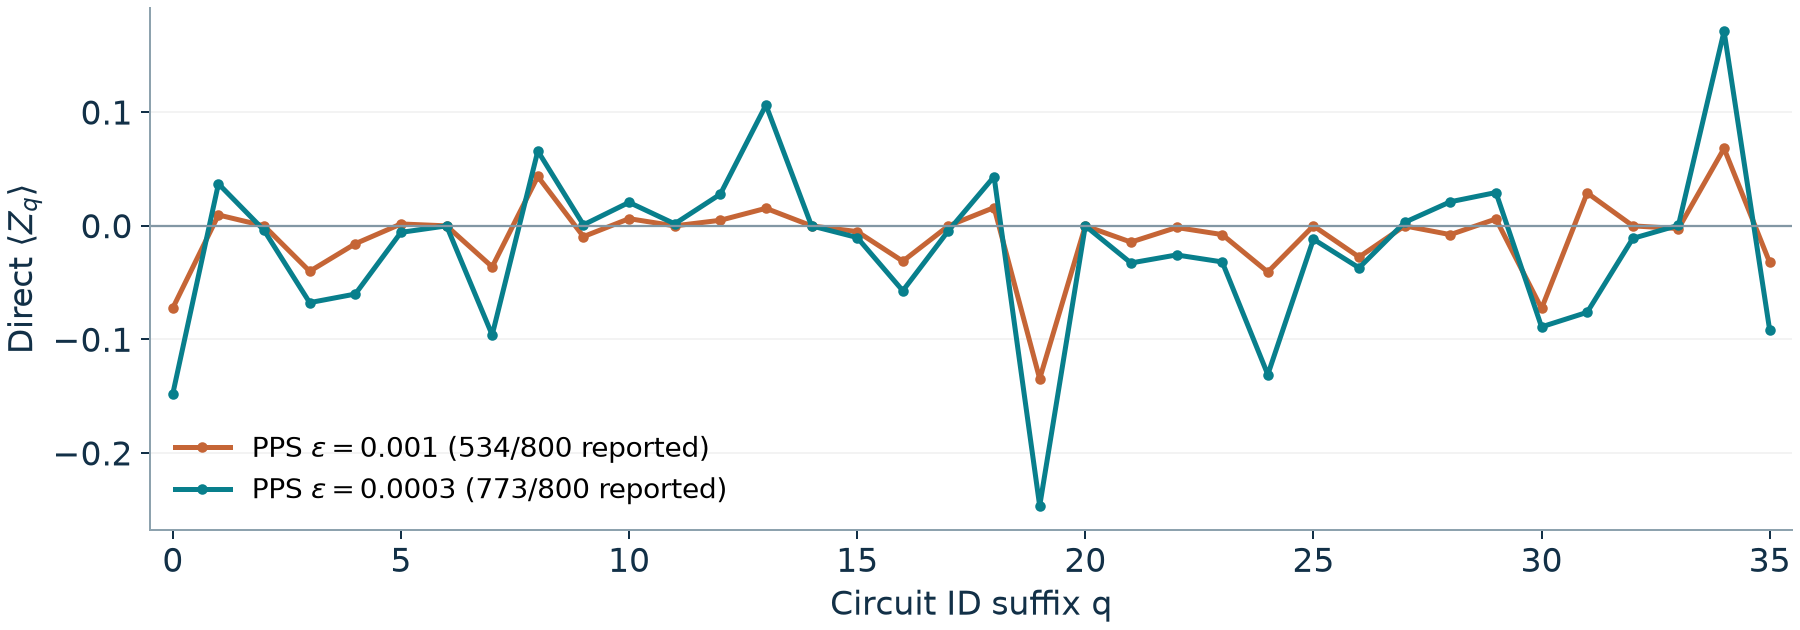
\includegraphics[width=\linewidth]{g3_values.png}
\column{.25\textwidth}
\vspace{.12cm}
{\Large\color{orange}534/800}\par
{\small $\varepsilon=0.001$; 9 zeros}\par\vspace{.3cm}
{\Large\color{teal}773/800}\par
{\small $\varepsilon=0.0003$; 3 zeros}\par\vspace{.35cm}
{\small\bfseries +239 reported points}\par\vspace{.18cm}
{\scriptsize The two saved vectors have $\rho=0.89169$; this compares approximations, not either one with the hidden answer.}
\end{columns}
\source{Hash-checked CSVs and receipts in \texttt{submissions/teammates/teammate-1/G3/}; figure from \texttt{render\_figures.py}.}
\end{frame}

\begin{frame}{G4: a zero score and a later PPS result}
\eyebrow{MPS $\chi=32$: accepted, user-reported 0/1000; a teammate's PPS: reported 133/1000}
\begin{columns}[T,onlytextwidth]
\column{.70\textwidth}
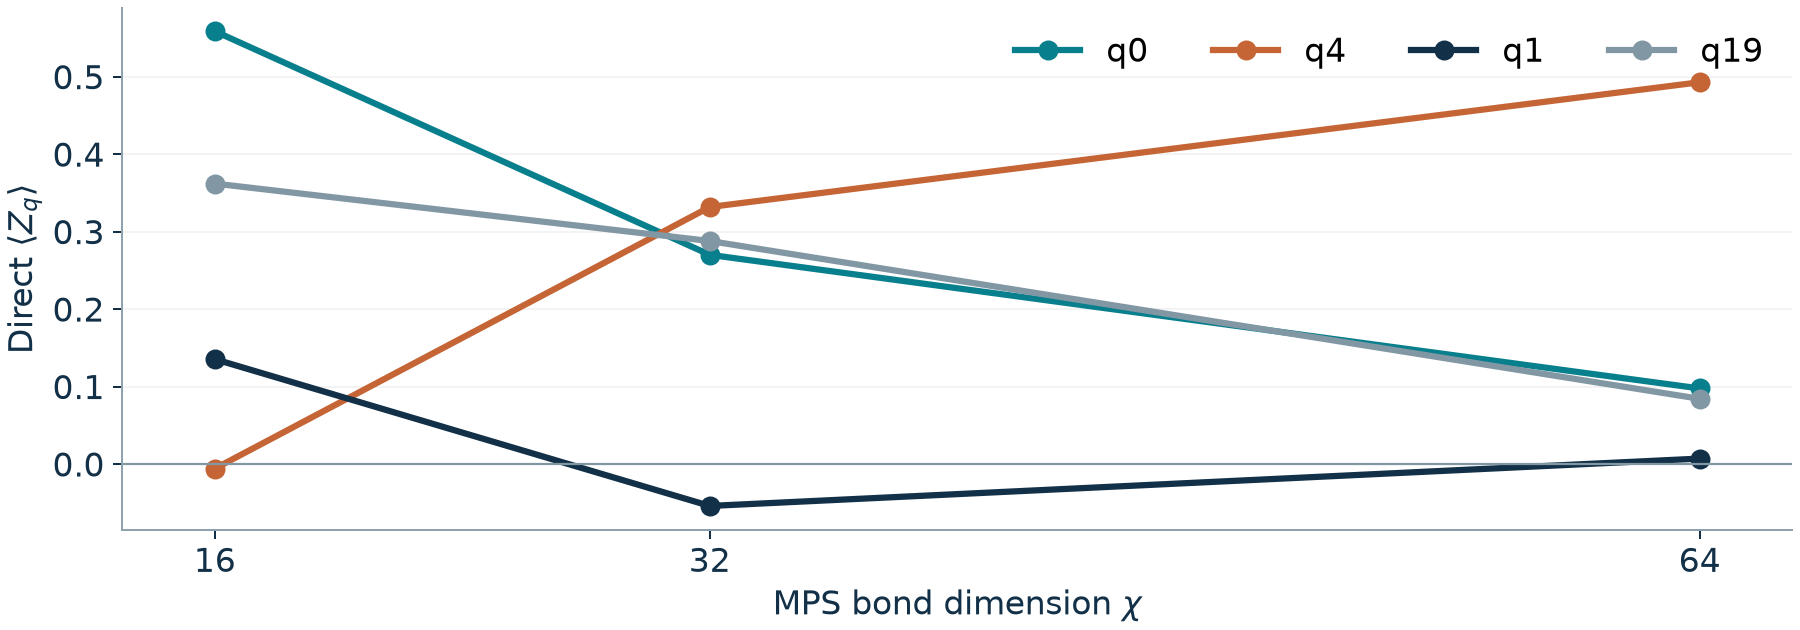
\includegraphics[width=\linewidth]{g4_trends.png}
\column{.27\textwidth}
\small
Four targeted CPU rows at $\chi=16,32,64$ changed differently. q1 reverses direction; q19's latest change grows about 2.75-fold.\par\vspace{.25cm}
On ten matched $\chi=16/32$ rows, the affine residual retains 26.19\% of centered energy; 12 of 45 pairs reverse order.
\end{columns}
\vspace{.12cm}
\caveat{Level-1 PPS q4 stayed zero as compute grew 33.4-fold. A teammate's later level-3 PPS vector had four zeros and a reported 133/1000, but q37 still moved at finer precision. These are different accounts and settings.}
\source{\texttt{submissions/G4/README.md}; \texttt{reports/g4\_partial\_trend\_review.json}; a teammate's G4 receipt.}
\end{frame}

\begin{frame}{A decision is useful if its outcome changes the next step}
\eyebrow{What we now do with a limited time and compute budget}
\begin{columns}[T,onlytextwidth]
\column{.53\textwidth}
\small
\begin{enumerate}
\item Reuse complete evidence. A teammate's exact G1 vector avoided 30 repeated runs.
\item Test representation and informative rows before increasing precision everywhere.
\item Compare signed changes, shape residuals, job cost, and elapsed time. Record why work stops.
\end{enumerate}
\column{.43\textwidth}
\begin{block}{Live evidence check}
\texttt{python writeup/slides/}\par\texttt{render\_figures.py --verify-only}
\end{block}
\small This reads saved files, checks G3 hashes and ID coverage, and prints the G3, S2, and G4 comparisons shown here. It does not call a simulator or the BlueQubit service.
\end{columns}
\vspace{.18cm}
\small A matched G4 q0 GPU trial saved 10.25 seconds of elapsed time for \$0.20. Hardware choice depends on the actual workload.
\par\vspace{.12cm}
\small\color{muted}Next test: under a fixed budget, can a broader G4 panel select a useful complete refinement? We have not compared this policy with another allocation rule under equal budgets.
\source{\texttt{writeup/main.tex}; \texttt{reports/gpu\_matched\_pilot.json}; \texttt{render\_figures.py}.}
\end{frame}

\appendix
\begin{frame}{Evidence map for questions}
\small
\begin{tabular}{@{}p{.23\textwidth}p{.69\textwidth}@{}}
\toprule
Claim & Saved source \\
\midrule
Pre-challenge design & \texttt{8fac5d9:estimation\_workflow\_v0.md} \\
Scoring and attribution & \texttt{docs/results.md}; \texttt{submissions/README.md} \\
S2 extrapolation test & \texttt{reports/extrapolation\_rejection.json} \\
G2 progression & \texttt{submissions/G2/README.md}; linked CSVs and feedback \\
G3 threshold comparison & a teammate's v2/v3 CSVs and receipts; \texttt{render\_figures.py} \\
G4 failure and diagnostics & \texttt{submissions/G4/README.md}; \texttt{runs/jobs.csv} \\
Resource tradeoff & \texttt{reports/gpu\_matched\_pilot.json}; \texttt{docs/workflow.md} \\
\bottomrule
\end{tabular}
\vspace{.25cm}
\caveat{The highest G2 reports lack a saved website receipt and row provenance. G4's zero is user-reported. A teammate's G3 results are teammate-reported with retained row records.}
\end{frame}

\end{document}
